\documentclass{article}  
\usepackage{graphicx}
\usepackage{url}
\usepackage{caption}
\usepackage{subcaption}
\usepackage{hyperref}

\title{Blocking-resistant communication through high-value web services}
\author{David Fifield, Chang Lan}

\begin{document}

\maketitle

\begin{abstract}
We describe meek, a blocking-resistant Internet communication system for censorship circumvention.
meek uses HTTP as a mechanism for transporting data, but it is not a steganographic HTTP transport;
rather, it relies on HTTPS to hide the contents of communications from a censor.
Communications are proxied through a web service that may itself be blocked by the censor:
``domain fronting''---in which the domain name used in the (censor-visible)
DNS request and TLS server name extension doesn't match the name in the (censor-invisible)
HTTP host header---enables communication that is apparently with an allowed host
but actually with a forbidden host.

Though HTTPS frustrates blocking by hiding the underlying communication,
differences in TLS implementations give rise to distinguishing features
that may be used to block circumvention traffic.
We describe how we use a web browser as a tool for making HTTPS requests,
so that the TLS signature of circumvention traffic resembles that of ordinary web browsing.
We present other, more subtle traffic characteristics that may enable blocking,
and identify potential countermeasures to such blocking.

We describe our experience implementing meek as a pluggable transport for Tor,
and the results of an initial experimental deployment.
\end{abstract}

\section{Introduction}

% VPN arms race We seek to build a system that remains difficult to block even
% after it has many users.

\ldots

The fact that we tunnel inside HTTPS greatly eases the steganography problem.
It's not necessary to generate plausible HTTP, only plausible TLS.
TLS payloads are encrypted, and to a first approximation all encrypted payloads look alike.
We need only make sure that the TLS handshake and other meta-attributes of the connection are not uniquely fingerprintable.
Section~\ref{sec:browserextension} describes the use of a web browser extension as a instrument for making HTTPS requests,
so things like the TLS handshake, DNS lookup, and TCP connection reuse match those of a browser as closely as possible.
Of course, there are more subtle considerations that go into
making a circumvention HTTPS stream look like an allowed HTTPS stream,
things like packet size and timing, and duration of TCP connections.
These additional considerations are the subject of Section~\ref{sec:trafficstatistics}.

Most of the discussion in this paper will use the specific example of the
Google frontend server as a front for App Engine.
App Engine is the system on which we have based our deployment,
and it suffices to illustrate the concept of domain fronting.
There are other systems, discussed in Section~\ref{sec:otherservices}
that can be substituted for App Engine, with few or no modifications.
When an example talks about ``App Engine,'' the reader may instead think
of other systems such as the CloudFlare content delivery network.

The confidentiality provided by HTTPS

Alternate domain fronting: use just an IP (no DNS and no SNI).

\section{Background and related work}

% In response to Internet censorship, many research papers and pragmatic systems
% such Freegate, Psiphon, and Lantern have explored the design space of censorship
% circumvention. All these schemes are based on a simple idea: deploy a set of
% proxies outside the censor's domain, and let the user connect to one of them
% which can pass data on to the true destination for the user.

% I'm thinking of recasting this as three challenges:
%  1. Content blocking.
%  2. Endpoint blocking.
%  3. Active scanning.
% We have something to say for all three and related work falls into one or
% more of those categories.
%
% "Cover your ACKs" talks about "unobservability" and "unblockability," maybe
% isomorphic to our "blocking by content" and "blocking by endpoint."

Broadly speaking, there are two main challenges to proxy-based circumvention:
blocking by content and blocking by endpoint.
Blocking by content means that the censor inspect packet or flow payloads,
looking, for example, for forbidden protocols or keywords.
Content-based blocking is countered by obfuscation:
making circumvention traffic difficult to distinguish
from traffic the censor wishes to allow.
Blocking by endpoint means that the censor forbids all communication with certain
network addresses, whatever the content of the communication.
The challenge of endpoint blocking is met by making it difficult for the censor to learn proxy addresses;
by making it difficult to scan for proxies;
by having sufficiently many proxies;
or by colocating proxies with high-value services, to block which would incur collateral damage.
Effective proxy-based circumvention requires that both these challenges be addressed.

Traffic obfuscation has been approached in many different ways,
which may be classified into two general techniques.
The first technique is to look unlike
anything forbidden by the censor; that is, fail to match a blacklist. The second is
to resemble a protocol that is explicitly allowed by the censor; that is, match a whitelist.
Falling into the first category are ``look-like-nothing'' transports whose
payloads are indistinguishable from a uniformly random byte stream.
Classic example of look-like-nothing
protocols are obfs2~\cite{obfs2} and its successor obfs3~\cite{obfs3},
which have been Tor's go-to pluggable transports since early 2012~\cite{obfsproxy-arms-race}.
ScrambleSuit~\cite{scramblesuit} is like obfs3 in the
content of its payloads, but it takes additional steps to obscure its traffic signature
(packet lengths and timing), and is designed to resist active scanning for proxies
(the proxy server remains silent until the client proves knowledge of a shared
secret).

The other category of obfuscation contains transports that take the steganographic approach: look like
something the censor doesn't block. StegoTorus~\cite{stegotorus}
encodes traffic to look like a cover protocol, such as unencrypted HTTP,
using special-purpose encoders.
Code Talker
Tunnel (formerly called SkypeMorph)~\cite{skypemorph} mimics a Skype video call.
FreeWave~\cite{freewave} encodes a digital stream into an acoustic signal
and sends it over VoIP to a proxy which decodes and forwards it to the destination.
fteproxy~\cite{fte} uses format-transforming encryption to encode data into strings that match a given regular expression,
in order to match a firewall's whitelist or avoid matching a blacklist.

Houmansadr et~al.~\cite{parrot} evaluate ``parrot'' systems that imitate a particular implementation of a protocol
and conclude that unobservability by imitation is a ``fundamentally
flawed approach.''
To fully mimic a complex and sometimes proprietary protocol like Skype
is difficult in that the system must imitate not only the protocol's normal operation, but also its reaction to errors,
its typical traffic patterns, and quirks of common implementations.
Geddes et~al.~\cite{acks}
demonstrate that even non-parrot systems may be vulnerable to
attacks that disrupt covert communication while having little effect
on legitimate traffic. Their examination is specific to VoIP protocols,
where packet loss and duplication are acceptable. The censor may
deliberately drop or inject ACKs in order to disrupt the covert channel, without causing
much collateral damage.


The other grand challenge of proxy-based circumvention is endpoint blocking,
against which there have been a few approaches proposed.
Tor has long faced the problem of its entry relays being blocked. The list of
relays is public, so it easy to block all of them by IP address. Tor
bridges~\cite{tor-blocking} are relays that are not universally known, intended
to serve as entry points for censored users. A database of bridges (BridgeDB) seeks to
provide a few secret bridges to anyone who asks, while at the same time making it
difficult to learn the entire list.
The database is accessible over HTTPS and email.
The HTTPS interface requires solving a captcha,
and the email interface responds only to addresses from certain providers, like Gmail,
that have defenses against bulk account creation.
BridgeDB has the feature that repeated queries from the same address
(IP subnet or email address) will receive the same small set of bridges.
Its resistance to enumeration therefore depends both on
having a large number of potential bridges,
and on the censor not being able to control large numbers of IP and email addresses.
BridgeDB is capable of distributing
the addresses of obfsproxy and ScrambleSuit bridges.
The combination
of careful bridge address disbursement and obfuscated protocols
gives Tor's system a realistic claim to addressing both challenges of proxy-based circumvention.
Address distribution appears to be the weaker side of the defense,
as evidenced by real-world censors' apparent preference for
blocking bridge addresses over real-time deobfuscation~\cite{foci12-winter}.

Flash proxy~\cite{flashproxy} attempts to address endpoint blocking by
conscripting web users as temporary proxies. Proxies last only as long as a web
user stays on a page, so the pool of proxies is constantly changing;
even if one of them is blocked, there will soon be another to replace it.
Flash proxy's approach to endpoint blocking is in a sense
the opposite of ours: where flash proxy uses cheap, disposable, individually blockable proxies,
we use just one high-value proxy, which shares its fate with network
infrastructure that is expensive to block.
A quirk of the browser proxy model is that the proxy connects to the client rather than the other way around.
The client must be able to receive a TCP connection; in particular it
may not be behind network address translation~(NAT), which limits flash proxy's usefulness.
Flash proxy itself does nothing to defend against content blocking.
Connections between censored clients and browser-based proxies use
WebSocket, a meta-protocol running on TCP,
but inside the WebSocket framing is the ordinary Tor protocol.
There exists a prototype transport that attempts to get both
content-based and endpoint-based blocking resistance by obfuscating traffic
with obfsproxy before sending it through flash proxy~\cite{obfs-flash}.
However it is limited because it is not
possible to obfuscate the outermost WebSocket layer;
the censor could decide simply to block all WebSocket.

% Lantern
% Psiphon
% Infranet
% Freegate
% Ultrasurf
% Dust

A technique known as OSS~\cite{oss} (for
``online scanning service'') bounces data
through third-party web services that are capable of making HTTP requests.
For example, a censored client may ask a translation service to
translate a web page at \begin{NoHyper}\url{http://proxy.example.com/...}\end{NoHyper},
where ``\begin{NoHyper}\url{...}\end{NoHyper}''
stands for the data payload that the client wishes to send---data are embedded in the URL.
Simply by making the HTTP request, the service sends the client's message.
The client cannot rely on being able to receive the response to its message in an HTTP response,
because online scanning services do not in general
return unmodified the contents of the page they are ordered to retrieve.
The translation service, for example, returns the page in another language.
For this reason, the server sends a response message by making
another reflected HTTP request back to the client, through the same OSS or a different one.
The need for the client to receive a connection means that OSS has the same problem with NAT that flash proxy does.
The NAT aspect is the most important way in which our work improves on OSS.
App Engine is effectively an unblockable OSS that we fully control.
We can ensure that reflected HTTP bodies are unmodified, and therefore use them to carry traffic
without having to connect to the client.

Decoy routing~\cite{decoyrouting} is a technique that puts
proxies in the middle of network paths, rather than at the endpoints.
Realizations of the decoy routing idea include Telex~\cite{telex}
and Cirripede~\cite{cirripede}.
Decoy routing asks friendly ISPs to deploy special software on routers that lie
between censored users and uncensored Internet destinations.
Circumvention traffic is ``tagged'' in a way that is detectable only
by decoy routers, and not by the censor.
On receiving a tagged communication, the decoy router shunts it away from its apparent destination
and toward the censored destination requested by the client.
Our work is conceptually similar to decoy routing,
though the action happens at the application layer rather than the network layer.
Both systems use a piece of network infrastructure as a decoy to redirect certain flows:
in decoy routing it is an ISP router; for us it is the front domain.
Both tag flows in a way that is visible only to the decoy router:
in decoy routing a tag may be, for example, a hash embedded in the TLS client randomness;
for us it is the HTTP Host header, encrypted within an HTTPS stream.
Decoy routing generally requires the cooperation of large, centrally located
router operators,
whereas we only need to buy web application hosting.

CensorSpoofer~\cite{censorspoofer}
decouples the upstream and downstream channels.
The client sends upstream data to the CensorSpoofer proxy over a low-bandwidth covert channel such as email.
At the same time, the client pretends to have an innocuous communication (such as a VoIP call) with an unblocked dummy host.
The CensorSpoofer proxy sends encrypted UDP data back downstream to the client,
protecting its true IP address by spoofing the source of all its packets
so that they appear to come from the dummy host.
From the censor's point of view, the client is carrying on a conversation only with the dummy host.
If the dummy is blocked, another can be used in its place,
as the CensorSpoofer proxy's true IP address remains unknown.

\cite{ccs2012-decoys}
% Routing around decoys
A recent study~\cite{nodirectionhome} on AS
topology suggests that defeating decoy routing is likely to be expensive for the
censors, if the decoy routers are strategically deployed. Despite that decoy
routing is a sound technical approach, it is not clear whether ISPs are
willing to act against censors. However, the takeaway is that the
censors are unwilling to completely block day-to-day Internet access, which we
can take advantage of.

CloudTransport~\cite{cloudtransport}

Winter and Lindskog~\cite{foci12-winter} investigated how China's Great Firewall blocks Tor.
They confirmed an earlier discovery of Wilde~\cite{wilde} that the firewall identifies Tor relays using more than passive monitoring:
it actively probes destination addresses to see if they speak the Tor protocol, and if so,
blocks them for the future.
(At the time, the firewall identified potential Tor connections for future probing by looking for a distinctive
list of TLS ciphersuites---a failure of obfuscation.) %\cite{bug4744}
The discovery of Chinese active probing was the motivation for probing resistance in ScrambleSuit
and in our work.

GoAgent~\cite{goagent} is a direct inspiration for our system in its use of App
Engine and Host header--based domain fronting.
As in our system, traffic is fronted by the Google frontend server
and delivered to its destination by a specialized app running on App Engine.
GoAgent requires users to upload a personal copy of the server code to App Engine,
which harms usability but requires no central management
and enables users to stay within bandwidth limits that exist for unpaid apps.
GoAgent is an HTTP and HTTPS proxy only.
It works by encapulating a desired HTTP request, including URL and POST body, if any,
and uploading the request to App Engine.
The app unpacks the encapsulated request and directly requests the desired URL using
App Engine's URL-fetching API.
The design is simple but has disadvantages, stemming from the web app's
need to know what URL to request.
In order to proxy HTTPS, the local GoAgent proxy program does a benign man-in-the-middle
attack on the browser, which must have previously trusted the GoAgent CA certificate.
The local proxy program decrypts the HTTPS in order to read from it the HTTP request including the URL.
When the response comes back, the local proxy re-encrypts it under its own key.
End-to-end security is lost; an attacker positioned at the web app
is able to observe and modify all traffic.
In our system, such an attacker may only deny service or perform traffic analysis on ciphertext.
Additionally, we allow proxying of any TCP-based traffic, not only HTTP.
According to a May 2013 survey~\cite{collateral-freedom},
GoAgent was the circumvention tool most used in
China, with 35\% of survey respondents having used it in the previous month.
This figure is higher than that of paid~(29\%) and free VPNs~(18\%), and far
above that of other special-purpose tools like Tor~(2.9\%) and Psiphon~(2.5\%).
Users identified reliability, speed, and ease of installation as the most important features of a circumvention tool.

% CORDON? Say how meek would be classified in it?

\section{Threat model}

The censor is able to inspect all traffic that passes through
the censorship boundary and block or allow it at will.
The censor is able to actively scan for proxies, and issue followup
connections to hosts that clients connect to, in order to determine
whether they are proxies.
The censor may block the web host on which the reflector web app runs,
but it must allow access to some domain that can front for it.
In our deployment using App Engine, the censor may block appspot.com,
but must allow www.google.com (or its IP address, or some other domain
that goes through the frontend server).

The censor must operate at line rate; that is,
it must not delay traffic unduly while deciding whether to allow it.
This consideration is one facet of the censor's sensistivity to
collateral damage caused by false positives:
mistakenly blocking or degrading non-circumvention traffic causes the censor
to incur some penalty, just as mistakenly allowing circumvention traffic does.
The censor must allow TLS connections; meek does not try to look like plaintext.

The user's computer, the third-party infrastructure (e.g., Google), and the Tor bridge
are all uncontrolled and uncompromised by the censor.
The user has a way to get a copy of the necessary client programs.

\section{Architecture}

\cite{pt}

\begin{figure}
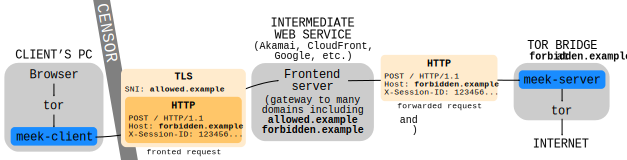
\includegraphics[width=\linewidth]{architecture}
\caption{
System architecture.
The Google frontend server is the server that dispatches requests to different services depending on the Host header.
Components that are new in our system are outlined in blue.
The ``Google infrastructure'' block may be replaced by other infrastructure that supports domain fronting.
}
\label{fig:architecture}
\end{figure}

\section{Making the TLS handshake indistinguishable}
\label{sec:browserextension}

Two big things: list of ciphersuites and extensions.

% Examples of how handshakes differ; e.g., OpenSSL versus NSS,
% and non-browser NSS versus browser NSS.

\begin{figure}
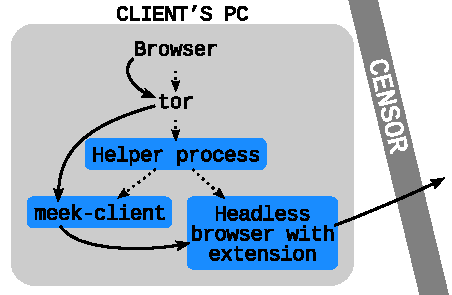
\includegraphics{browser-architecture}
\caption{
Client architecture including a browser extension for TLS camouflage.
Dashed lines show the process hierarchy.
Solid lines show the flow of outgoing communication.
The headless instance of the browser runs in the background and is invisible to the user.
This figure is a detailed view of the ``User's PC'' component of Figure~\ref{fig:architecture}.
}
\label{fig:browser-architecture}
\end{figure}

\section{Making traffic characteristics indistinguishable}
\label{sec:trafficstatistics}

The censor cannot sniff the content of communications or infer the existence of meek traffic 
from packet \emph{data}, 
since the communication is encrypted inside the TLS session, and we have devoted large efforts 
in hiding TLS handshake fingerprints. However, it is still possible that the censor can detect 
the existence of meek traffic according to the \emph{meta-data}, i.e. traffic characteristics. 
We studied a collection of traffic characteristics and evaluated their possibilities of becoming
the censor's interest. Specifically, we considered three characteristics: 1) payload length of
TCP packets, 2) number of concurrent HTTPS connections, 3) HTTPS connection lifetime. To collect 
the traffic trace of meek, we browsed the Alexa top 500 websites sequentially using the Tor Browser Bundle
and dumped the traffic trace from 
the network interface. We ensured only the browser can successfully access the network by setting
up the \texttt{iptables} firewall so that packets from other processes will be dropped. We also 
obtained a 10-minute sample of normal HTTPS traffic trace from LBL. The trace is 983 MB in total. We also
specifically extracted the traffic between LBL and Google. Since the trace only has packet headers, we 
cannot extract the domain information. However, the \texttt{TXT} DNS records of the domain 
\texttt{\_netblocks.google.com} shows the IP address blocks that belongs to Google. Therefore, we 
determine whether a flow is from or to Google by examining the address in the IP header. For this
study we are only interested in Google traffic, because the censor will be mostly likely to compare
suspected meek traffic with normal Google traffic. This part of the trace is 312 MB in size. 


% 1. TCP payload length
% 2. Number of concurrent connections
% 3. Connection Lifetime

% Conclusion:
% 1. long-lived connections with bulk data transfer may be suspicious
% 2. Distribution of packet sizes 

\begin{figure}
\centering
\begin{subfigure}[b]{0.5\textwidth}
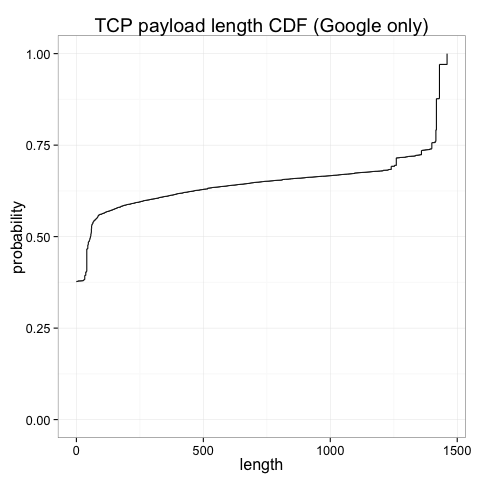
\includegraphics[width=\textwidth]{figs/datalen-google-cdf.png}
\caption{Normal Google Traffic}
\label{fig:len:lbl}
\end{subfigure}%
%add desired spacing between images, e. g. ~, \quad, \qquad, \hfill etc.
%(or a blank line to force the subfigure onto a new line)
\begin{subfigure}[b]{0.5\textwidth}
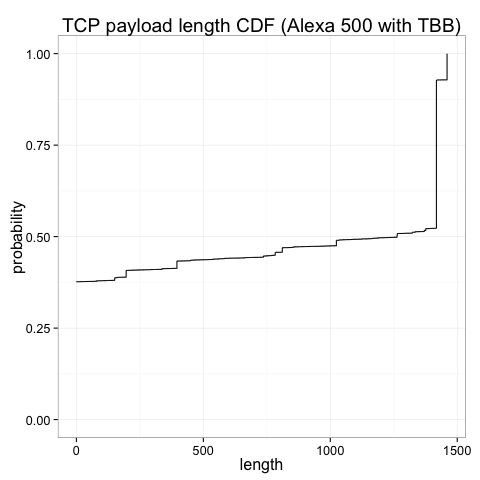
\includegraphics[width=\textwidth]{figs/datalen-tbb-cdf.png}
\caption{Traffic Using meek}
\label{fig:len:meek}
\end{subfigure}

\caption{TCP packet payload size distribution}
\label{fig:len}
\end{figure}

\paragraph{TCP payload length}
Figure \ref{fig:len} shows the payload size distribution of normal Google traffic and meek traffic. Both
figures exhibit a significant amount of packets with no payload. Most likely these packets are TCP SYN and ACK
packets. Figure \ref{fig:len:lbl} is the distribution of normal traffic, which indicates a large portion
of small-sized packets. While in the distribution of meek traffic shown in Figure \ref{fig:len:meek}, most packets
are large packets ranging from 1400B to 1500B. 

Recall that we use browsers to handle HTTPS connections for meek in order to hide TLS handshake characteristics.
Browsers also apply techniques like HTTP pipelining to improve performance. Since meek is always communicating with
the same Google frontend server, the browser will keep the persistent TLS connection. In addition, small requests 
can be batched into a large chunk before being sent. This explains why large packets are mostly seen from the meek trace.
In contract, normal users may not have persistent connections to Google. For example, a user may search a keyword on
Google, click a result, and then close the tab that displays search results. The browser may close the 
connection immediately after the user leaves the Google web page. Next time the user browses Google search, the browser 
opens a new connection. In this case, small requests do not have such opportunity for batching.

These browser techniques improve performance, but also lead to unexpected risks. The censor may be aware of the 
deviation from the distribution of normal traffic. Additionally, the persistent connection itself can be a problem.
We thus investigated other related characteristics.

\begin{figure}
\centering
\includegraphics[width=0.7\textwidth, angle=270]{figs/connections-google.eps}
\caption{Histogram of each user's connections in the 10-minute window}
\label{fig:connections}
\end{figure}
%add desired spacing between images, e. g. ~, \quad, \qquad, \hfill etc.
%(or a blank line to force the subfigure onto a new line)
\begin{figure}
\centering
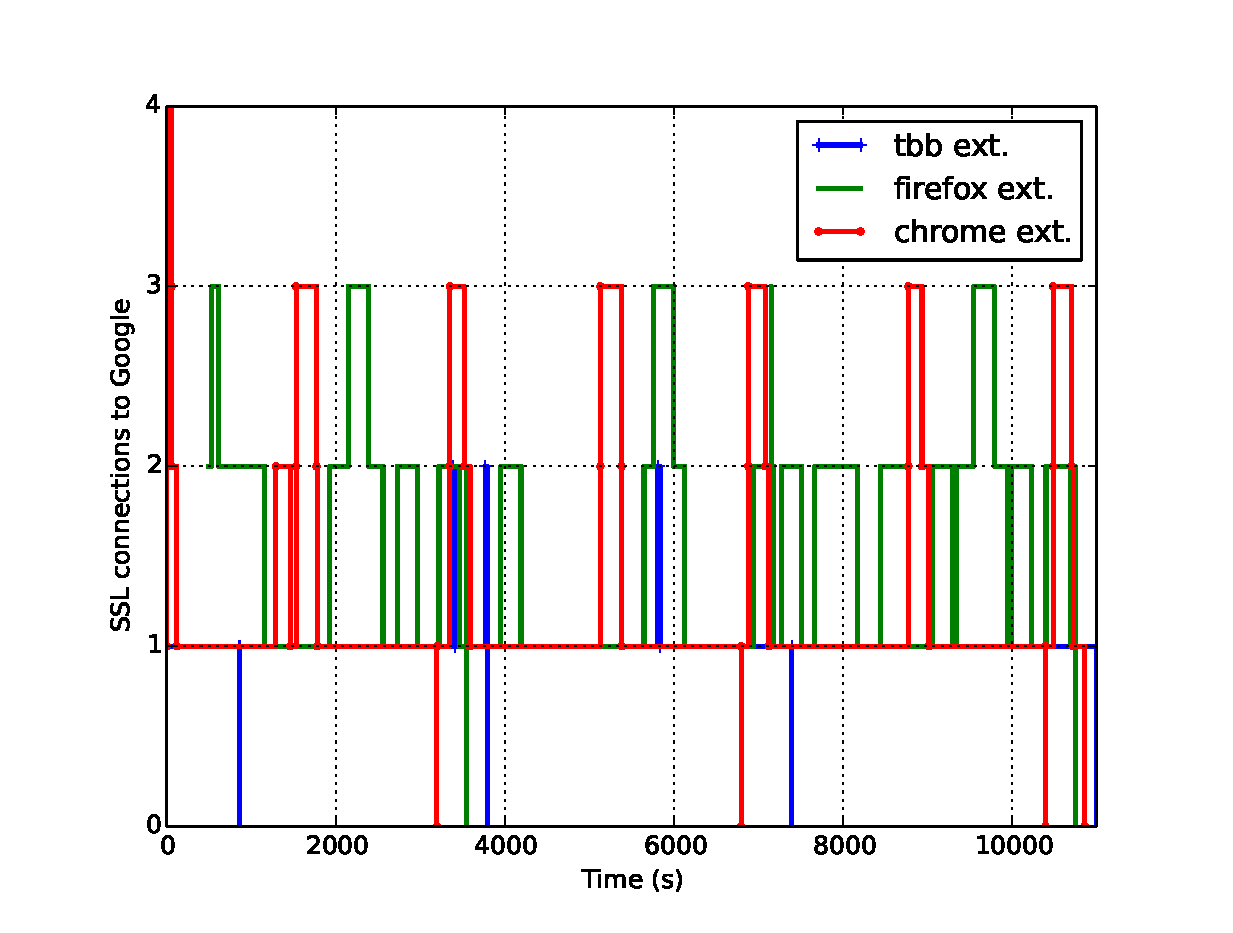
\includegraphics[width=0.8\textwidth]{figs/conns.eps}
\caption{Concurrent HTTPS connections over time. We measure the trace for the Tor Browser Bundle and Firefox/Chrome extensions.}
\label{fig:conconns}
\end{figure}

\paragraph{Concurrent connections}
Figure \ref{fig:connections} shows how many HTTPS connections to Google did a user make 
during the 10-minute measurement window.
There are 34,732 connections in total from 2,745 unique IPs. We observe that the majority of users have less than 
50 connections to the Google frontend server, and most of the numbers concentrate on 1 ~ 10. This is not unexpected
because a typical pattern of using Google is using the Google search as a stepping stone for other websites.

We measure the number of concurrent HTTPS connections during the automated browsing of Alexa
top 500 sites using three platforms: Tor Browser Bundle, Safari + Firefox extension, and Safari + Chrome extension.
Figure \ref{fig:conconns} shows the number over time. We can see that most of the time
the browser has one HTTPS connection to Google. Sometimes the browser may have more than one connection
due to background activities such as statistics reporting. In all cases the number of connections is always 
less than 5. We can conclude that the number of concurrent connections does not show distinct characteristics, as 
a small number of connections can be considered as a normal behavior.

\begin{figure}
\centering
\begin{subfigure}[b]{0.5\textwidth}
\includegraphics[height=\textwidth, angle=270]{figs/flowduration-google-cdf.eps}
\caption{Normal Google Traffic}
\label{fig:duration:lbl}
\end{subfigure}%
%add desired spacing between images, e. g. ~, \quad, \qquad, \hfill etc.
%(or a blank line to force the subfigure onto a new line)
\begin{subfigure}[b]{0.5\textwidth}
\includegraphics[height=\textwidth, angle=270]{figs/flowduration-tbb-cdf.eps}
\caption{Traffic Using meek (Notice the x-axis)}
\label{fig:duration:meek}
\end{subfigure}

\caption{Connection lifetime distribution}
\label{fig:duration}
\end{figure}

\paragraph{Connection lifetime}
We consider the connection lifetime as a potential weakness. Figure \ref{fig:duration:lbl} shows the 
connection lifetime distribution of normal traffic. Interestingly we can see the concentration on 
several discrete values: 60s, 120s, 180s, 240s. We hypothesize that it is due to the HTTP Keep-Alive 
timeout of different browsers and web services. Another important observation is the concentration on 
durations that exceed 600 seconds. Note that our trace only contains 10 minutes' data, therefore the concentration 
on 600 seconds does not reflect that these connections' actual duration is 600 seconds. Rather, 600 seconds
is the lower bound of their actual duration. Thus, we can conclude that only about 10\% connections last 
longer than 600 seconds.

The distribution of meek traffic, in contrast, is totally different. First, there are much fewer connections, which is 
consistent with the discussions above. Second, the durations are much longer if we notice the x-axis in Figure \ref{fig:duration:meek}. If there is not a case in which normal users also have such long connections when browsing Google, the 
censor can potentially block any long connections between users and Google. Even if this is the case, the
censor has to wait until a time threshold is reached. The user may already obtained the forbidden data she wants, or 
meek could simply restart a connection.

\paragraph{Conclusion} So far we have found two potential weaknesses: long-lived connections with bulk data transfer, 
and deviated distribution of packet sizes. To fundamentally fix these weaknesses we need to transform to the traffic into the normal-looking traffic. The problem is inherently difficult, because we need to know \emph{what} is normal traffic, i.e. what
is the model of normal traffic, which is an open problem. However, the arm-race game is symmetric; since finding a right
model is a difficult task for us, it is also difficult for the censor. Therefore, the censor can only find ad-hoc 
characteristics to block forbidden traffic, which are relatively easy to defend against. 

\section{Usage scenarios}

The default usage scenario has a single paid App Engine instance, publicly known and usable by anyone,
with software configured to use the public instance by default.
This way has the greatest usability because there is nothing to upload and nothing to configure.
The number of parties able to analyze users' traffic patterns is somewhat increased:
the path from user to bridge now includes Google and the app operators, not only the ISP and intermediate routers that were there before.
On the other hand, the bridge no longer gets to see users' IP addresses.
In effect, Google and the app become what Tor calls a ``guard node.''
Because Tor is encrypted and integrity-protected, neither Google nor the app operators
are able to read or alter users' communications, but being able to measure packet timings,
for example, is necessary for certain linking attacks.

Users are also free to upload their own personal copy of the App Engine code, as is done with GoAgent.
App Engine imposes bandwidth quotas on unpaid apps, but they are high enough to allow daily web browsing.
In this scenario, Google still has a privileged network position,
but the user's traffic is no longer visible to the operators of the public app instance.
% Outgoing HTTP requests include app id? As good as an IP address.

The code that runs on App Engine is very simple.
It just statelessly copies HTTP requests and responses.
Another usage scenario has the App Engine code ported to another language such as PHP,
so that it can be run in ordinary web hosting environments.
What you lose with a PHP app is Google's unblockability;
the censor may find and individually block the domains
This scenario is still interesting because there are so many places
where such an app can be run, with low cost and minimal setup.
Installing a PHP file on a web host environment is easier than setting up a Tor bridge or SOCKS proxy.
The URLs of PHP bridges could be distributed in a way like BridgeDB.

\section{Other third-party services}
\label{sec:otherservices}

A censor can block meek by blocking access to Google entirely.
To take such a step is extreme, because of its high collateral damage,
but it is not outside the realm of possibility.
% Cite when Google and Gmail were completely blocked temporarily.
We investigated how easily our system can be adapted to hard-to-block systems other than Google,
and found that CloudFlare, a content delivery network, in principle supports domain fronting.

CloudFlare provides the frontend of $X$ web sites, $Y$ of them supporting HTTPS~\cite{something}.
CloudFlare supports the domain fronting trick;
that is, it is possible that a request has one domain in the TLS layer
and another in the HTTP layer, and the CloudFlare server will transparently redirect it to proper place.
While we verified that domain fronting would work on CloudFlare,
we did not test deployment,
because when we asked we were told that our planned use would be against CloudFlare's terms of service.
CloudFlare hosts a number of HTTPS sites.
Choosing just one of them to be the front in TLS connections could cause
the innocent third-party domain to be censored even though it is not itself carrying any circumvention traffic.
To avoid this problem, the front can be simply a CloudFlare IP address,
with no SNI at all.
The censor then faces the choice of allowing circumvention traffic,
or else blocking a large number of popular unrelated web sites.

We were not able to make the system work with Amazon CloudFront nor Akamai.
% Dreamhost? Other HTTPS webhosts with PHP bridge?

\section{Security}

% Google can deanonymize you, because they are the first hop,
% and also often the last hop because of their popularity.

\section{Deployment}

We implemented meek as a Tor pluggable transport~\cite{pt}
and built experimental releases of the Tor Browser Bundle featuring meek.
The browser bundle includes Tor and a version of Firefox
called Tor Browser that is patched to defend against application-layer identity leaks.
Users need to download and run the bundle and select meek from the list of transports,
and then a browser window appears,
configured to use meek for circumvention and Tor for anonymity.
We announced our prototype bundles on Tor development mailing lists,
and from there they were picked up by Tor Weekly News on the Tor blog.

\begin{figure}
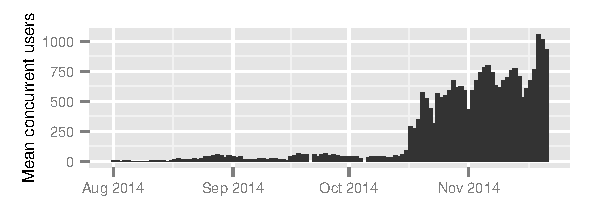
\includegraphics[width=\linewidth]{clients-meek}
\caption{Number of concurrent users using the meek transport,
as reported by the Tor Metrics Portal.
The gap between April~14 and April~22 is when the Tor bridge authority
was down because of the Heartbleed OpenSSL vulnerability~\cite{heartbleed}, and wasn't collecting statistics.}
\label{fig:clients}
\end{figure}

Figure~\ref{fig:clients} shows the number of concurrent users of meek between January and May~2014,
as reported by the Tor Metrics Portal~\cite{metrics-meek}.
The number of concurrent users is estimated by counting directory requests made over the transport~\cite{counting-daily-bridge-users}.
The drop to zero on May~8 coincides with the reinstallation of the Tor bridge used by meek.

We are running a paid instance of the web app on App Engine for use by the public.
The cost for bandwidth on App Engine is \$0.12 per gigabyte,
with one gigabyte free each day.
The total cost has so far been \$1.11, with bills of
\$0.09 in March,
\$0.73 in April,
and \$0.29 in May through May~12.

meek has a home page at
\url{https://trac.torproject.org/projects/tor/wiki/doc/meek}.
Our source code is in the Git repository at
\url{https://git.torproject.org/pluggable-transports/meek.git}.
As of version 0.5 (May~7, 2014), the source code consists of
about 800 lines of Go for the client programs,
400 lines for the server, and
100 lines for the intermediary web app.
Each of the browser extensions
(one for Firefox, one for Chrome)
is about 300 lines of JavaScript.

\section{Future work}

% Pipelining of requests.
% Put a diagram here showing serialized requests.
% Simple reliability layer, SEQ/ACK.
% Would be useful for Iran-like session cutoff, independent of meek.

\section{Acknowledgements}

tor-dev
tor-qa
George Kadianakis
Georg Koppen
Lunar
Yawning Angel
Vern Paxson
Nick Weaver

%%%%%%%

% HTTPS or not on the App Engine--bridge link.
% HTTPS obscures session ids, equivalent to obscuring TCP connections in other transports.
% Increases latency a lot: \approx 100 ms increased to \approx 350 ms when I tried it in March 2014.

\bibliographystyle{plain}  
\bibliography{meek}

\end{document}
